\documentclass[a4paper]{report}

\usepackage{amssymb, amsmath}
\usepackage{tikz}

\newcommand{\vens}{\ensuremath{v_{\mathrm{ens}}}}


\title{Replicating John Philip 1972}
\author{Nat Lund}

\begin{document}
\maketitle

The first known expression for an effective slip length appeared in 1972, in a paper in ZAMP by John R. Philip entitled ``Flows Satisfying Mixed No-Slip and No-Shear Conditions".

In the paper, John R. Philip says that the limit of
\begin{equation}
W_{3} = \Im \left[  
 \alpha^{-1} \cos^{-1} 
 \left\{ \frac{\cos(\alpha \Theta)}{\cos \alpha} \right\} - \Theta
   \right]
\end{equation}
as $y\rightarrow \infty$ is
\begin{equation}
W_{3} = \alpha^{-1} \ln \sec \alpha
\end{equation}

Let us prove this forthwith.
\vspace*{1em}

$\Theta = x + iy$ is a complex number, $\alpha$ is real.  Trig identities for \emph{complex} cosine and \emph{complex} exponential and log:
\begin{gather}
\arccos z = - i \ln (z + \sqrt{z^{2} - 1}) \\
\cos z = \frac{e^{iz}+e^{-iz}}{2} \\
e^{i \theta} = \cos \theta + i \sin \theta 
\end{gather}

\subsubsection*{Expand complex cosine term, dump negligible parts}

In Euler's formula $e^{i\theta} = cis(\theta)$, if $\theta$ is \emph{real}, then $e^{i \theta}$ traces out the unit circle in $\mathbb{C}$, with $\theta$ being the angle.
\begin{center}
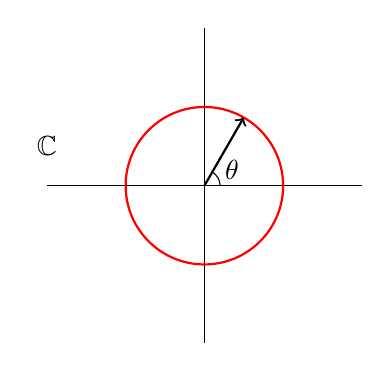
\begin{tikzpicture}
\draw (-2,0) -- ++ (4,0);
\draw (0,-2) -- ++(0,4);
\node at (-2,0.5) {$\mathbb{C}$};

\draw[thick, red] (0,0) circle (1cm);
\draw[thick,->] (0,0) -- ++(60:1);
\draw (0.2,0) arc  (0:60:2mm);
\node at (0.35,0.2) {$\theta$};

\end{tikzpicture}
\end{center}

This gives insight into the $\cos z$ function.  If $z$ is real, then $\frac{1}{2} e^{iz}$ and $\frac{1}{2} e^{-iz}$ are two vectors of length $\frac{1}{2}$ that cycle in opposite directions, with $z$ being the angle. Then $\cos z$ is the sum of the two vectors, which always ends on the real line between -1 and 1. 

\begin{center}
\begin{tikzpicture}
\draw (-4,0) -- ++ (8,0);
\draw (0,-2.5) -- ++(0,5);
\node at (-3,0.5) {$\mathbb{C}$};
\draw (4,0.1) -- ++(0,-0.2) node[below] {1};
\draw (-4,0.1) -- ++(0,-0.2) node[below] {-1};

\draw[thick, red, dashed] (0,0) circle (2cm);
\draw[thick, ->] (0,0) -- ++(45:2) -- ++(-45:2) node[below]{cos $z$};
\draw[thick, ->] (0,0) -- ++(45:2);
\node at (0.2,1)[right]{$\frac{1}{2} e^{iz}$};
\node at (2,1)[right]{$\frac{1}{2} e^{-iz}$};

\draw (0.3,0) arc  (0:45:3mm);
\node at (0.45,0.15) {$z$};

\draw[thick, dashed, ->] (0,0) -- ++(-45:2);
\draw (0.25,0) arc (0:-45:2.5mm);
\node at (0.45,-0.15) {$-z$};

\end{tikzpicture}
\end{center}

With this insight, it is useful to rewrite $\cos z$ as:
\begin{equation}
\cos (x + iy) = \frac{ e^{i(x+iy)}+e^{-i(x+iy)} }{2} =
\frac{ e^{ix - y} + e^{-ix + y} }{2} = 
e^{y} \frac{1}{2}e^{-ix} + e^{-y} \frac{1}{2} e^{ix}
\end{equation}

Then it is clear that $\cos (x + iy)$ is the sum of two rotating vectors in $\mathbb{C}$ with amplitudes $e^y$ and $e^{-y}$.  A consequence is that for large $y$, $e^y$ is \emph{very} large, while $e^{-y}$ is negligible, therefore $\cos (x + iy)$ is dominated by the vector $ e^{y} \frac{1}{2}e^{-ix} $.

\begin{center}
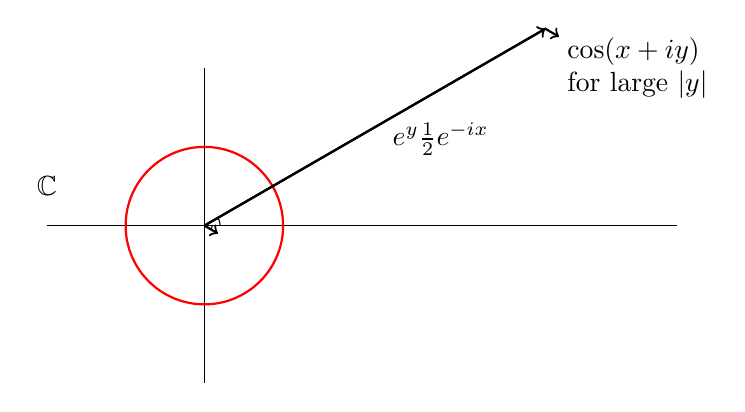
\begin{tikzpicture}
\draw (-2,0) -- ++ (8,0);
\draw (0,-2) -- ++(0,4);
\node at (-2,0.5) {$\mathbb{C}$};

\draw[thick, red] (0,0) circle (1cm);

\draw[thick,->] (0,0) -- ++(30:5) -- ++(-30:0.2);
\draw[thick,->] (0,0) -- ++(30:5);
\draw (0.2,0) arc  (0:30:2mm);
\draw[thick,->] (0,0) -- ++(-30:0.2);
\draw (0.1,0) arc (0:-30:1mm);

\node at (3,1.1) {$e^{y} \frac{1}{2}e^{-ix}$};
\node at (5.5,2)[align=left] {$\cos (x+iy)$\\ for large $|y|$};

\end{tikzpicture}
\end{center}

\begin{equation}
\text{Therefore} \quad \cos (x + iy) \to  \frac{e^{y} e^{-ix}}{2}
\quad \text{as} \quad y \to \infty
\end{equation}


The complex cosine term in J. R. Philip's expression is:
\begin{equation}
\left\{ \frac{\cos(\alpha \Theta)}{\cos \alpha} \right\} = 
\left\{ \frac{\cos(\alpha(x + iy)}{\cos \alpha} \right\} =
\left\{ \frac{\cos(\alpha x + i \alpha y)}{\cos \alpha} \right\}
\end{equation}
For any fixed real $\alpha$, as $y \to \infty$,
\begin{equation}
\left\{ \frac{\cos(\alpha x + i \alpha y)}{\cos \alpha} \right\} \to
\left\{ \frac{ e^{\alpha y} e^{-i\alpha x} }{2 \cos \alpha} \right\}
\end{equation}
The magnitude of this complex number tends to infinity as $y \to \infty$.

\subsubsection*{Express Arccos as Logarithm}

Using the identity $\arccos z = - i \ln (z + \sqrt{z^{2} - 1})$, $W_{3}$ becomes:
\begin{equation}
 W_{3} = \Im \left[  
 - i \alpha^{-1} \ln \left(
 \left\{ \frac{\cos(\alpha \Theta)}{\cos \alpha} \right\}
 + \sqrt{\left\{ \frac{\cos(\alpha \Theta)}{\cos \alpha} \right\}^{2} - 1} \right) 
  - \Theta  \right]
\end{equation}

As the magnitude of a complex number $z$ tends to infinity, subtracting 1 from it has a negligible effect. Therefore, as $y \to \infty$, $\sqrt{z^2 - 1} \to z$, and furthermore,
\begin{equation}
\text{For} \quad z = x + iy, \quad \ln(z + \sqrt{z^2 - 1}) \to \ln(2z)
\quad \text{as} \quad y \to \infty
\end{equation}
Hence,
\begin{equation}
W_3 \to 
\Im \left[  
 - i \alpha^{-1} \ln \left( 2
 \left\{ \frac{\cos(\alpha \Theta)}{\cos \alpha} \right\} \right) 
  - \Theta  \right]
\quad
\text{as}
\quad y \to \infty 
\end{equation}
%Since as $y \to \infty$
%\begin{equation*}
%2  \left\{ \frac{\cos(\alpha \Theta)}{\cos \alpha} \right\} \to
%\left\{ \frac{ e^{\alpha y} e^{-i\alpha x} }{\cos \alpha} \right\}
%\end{equation*}
Substituting for the $\cos$ expression in the limit, we have
\begin{align}
\lim_{y \to \infty} W_3 =
 \Im \left[  
 - i \alpha^{-1} \ln \left(
\frac{ e^{\alpha y} e^{-i\alpha x} }{\cos \alpha}
 \right) 
  - \Theta  \right] 
%\end{equation}
\\
%\begin{equation}
 =
 \Im \left[  
 - i \alpha^{-1} \ln \left( e^{\alpha (y - ix)}
\frac{ 1 }{\cos \alpha}
 \right) 
  - \Theta  \right] 
\end{align}

Apply the logarithm law $\log xy = \log x + \log y$, giving:
\begin{equation}
\lim_{y \to \infty} W_3 =
 \Im \left[  
 - i \alpha^{-1} \left( \ln  e^{\alpha (y - ix)} +
\ln \left\{ \frac{ 1 }{\cos \alpha} \right\}
 \right) 
  - \Theta  \right] 
\end{equation}
Apply the log definition: $\ln e^z = z$:
\begin{align}
\lim_{y \to \infty} W_3
=   \Im \left[  
 - i \alpha^{-1} \left( \alpha (y - ix) +
\ln \left\{ \frac{ 1 }{\cos \alpha} \right\}
 \right) 
  - \Theta  \right] 
\\
=  \Im \left[  
 - i \alpha^{-1} \alpha (y - ix) 
 - i \alpha^{-1} \ln \left\{ \frac{ 1 }{\cos \alpha} \right\}
  - \Theta  \right] 
\\
= \Im \left[  
  (i^2 x - iy) 
 - i \alpha^{-1} \ln \left\{ \frac{ 1 }{\cos \alpha} \right\}
  - \Theta  \right]
\\
= \Im \left[  
  -(x + iy) 
 - i \alpha^{-1} \ln \left\{ \frac{ 1 }{\cos \alpha} \right\}
  - \Theta  \right]
\\
= \Im \left[  
  - \Theta
 - i \alpha^{-1} \ln \left\{ \frac{ 1 }{\cos \alpha} \right\}
  - \Theta  \right]
\\
= \Im \left[  
  - 2 \Theta
 - i \alpha^{-1} \ln \left\{ \frac{ 1 }{\cos \alpha} \right\}
      \right]
\\
= \Im \left[  
  - 2x - 2iy
 - i \alpha^{-1} \ln \left\{ \frac{ 1 }{\cos \alpha} \right\}
      \right]
\\
= - 2y
  - \alpha^{-1} \ln \left\{ \frac{ 1 }{\cos \alpha} \right\}
\end{align}

The problem is the minus sign in $\arccos z = - i \ln (z + \sqrt{z^{2} - 1})$.  Without it, all is well.

UPDATE:  The minus sign appears to be just a convention.  Adopting the other convention fixes the problem.

\subsubsection*{Alternative Square Root Sign.}

We have 
\begin{equation}
\text{For} \quad z = x + iy, \quad \ln(z + \sqrt{z^2 - 1}) \to \ln(2z)
\quad \text{as} \quad y \to \infty
\end{equation}
but there is another possibility.
\begin{align}
z + \sqrt{z^2 - 1} = z + \sqrt{z^2(1 - \frac{1}{z^2})} \\ \approx
 z + \sqrt{z^2(1 - \frac{1}{z^2} + \frac{1}{4z^4})} \\
 = z + \sqrt{z^2(1 - \frac{1}{2z^2})^2} \\
 = z \pm z (1 - \frac{1}{2z^2}) \\
\end{align}
\begin{gather}
z + \sqrt{z^2 - 1} = z + z(1 - \frac{1}{2z^2}) = 2z - \frac{1}{2z^2} \\
\text{or} \\
z + \sqrt{z^2 - 1} = z - z(1 - \frac{1}{2z^2}) = z - z + \frac{1}{2z^2} = \frac{1}{2z^2}
\end{gather}

Thus, we now try
\begin{equation}
\ln ( \frac{1}{2z^2} ) = \ln( (\sqrt{2} z )^{-2} ) = -2 \ln (\sqrt{2} z)
\end{equation}
Hence,
\begin{equation}
 W_{3} = \Im \left[  
 - i \alpha^{-1} \ln \left(
 \left\{ \frac{\cos(\alpha \Theta)}{\cos \alpha} \right\}
 + \sqrt{\left\{ \frac{\cos(\alpha \Theta)}{\cos \alpha} \right\}^{2} - 1} \right) 
  - \Theta  \right]
\end{equation}
is equal to:
\begin{equation}
 W_{3} = \Im \left[  
 2 i \alpha^{-1} \ln \left( \sqrt{2}
 \left\{ \frac{\cos(\alpha \Theta)}{\cos \alpha} \right\}
                     \right) 
  - \Theta  \right]
\end{equation}
Substitute in the cosine expression:
\begin{align}
 W_{3} = \Im \left[  
 2 i \alpha^{-1} \ln \left( \sqrt{2}
\frac{ e^{\alpha y} e^{-i\alpha x} }{2 \cos \alpha} 
                     \right) 
  - \Theta  \right]
\\
= \Im \left[  
 2 i \alpha^{-1} \ln \left( \sqrt{2}^{-1} e^{\alpha(y - ix)}
\frac{1}{\cos \alpha} 
                     \right) 
  - \Theta  \right]
\end{align}
Apply logarithm law $\log xy = \log x + \log y$
\begin{equation}
W_3 = \Im \left[  
 2 i \alpha^{-1}  \left( \ln ( \sqrt{2}^{-1}) + \ln e^{\alpha(y - ix)}
+ \ln \left\{ \frac{1}{\cos \alpha} \right\}
                     \right) 
  - \Theta  \right]
\end{equation}
Apply log definition:
\begin{align}
W_3 = \Im \left[  
 2 i \alpha^{-1}  \left( \ln ( \sqrt{2}^{-1}) + \alpha(y - ix)
+ \ln \left\{ \frac{1}{\cos \alpha} \right\}
                     \right) 
  - \Theta  \right]
\\
= \Im \left[  
 2 i \alpha^{-1} \ln ( \sqrt{2}^{-1}) + 2 i \alpha^{-1} \alpha(y - ix)
+ 2 i \alpha^{-1} \ln \left\{ \frac{1}{\cos \alpha} \right\}
  - \Theta  \right]
\\
= \Im \left[  
 2 i \alpha^{-1} \ln ( \sqrt{2}^{-1}) + 2 (x + iy)
+ 2 i \alpha^{-1} \ln \left\{ \frac{1}{\cos \alpha} \right\}
  - \Theta  \right]
\\
= \Im \left[  
 2 i \alpha^{-1} \ln ( \sqrt{2}^{-1}) + 2 \Theta
+ 2 i \alpha^{-1} \ln \left\{ \frac{1}{\cos \alpha} \right\}
  - \Theta  \right]
\\
= \Im \left[  
 2 i \alpha^{-1} \ln ( \sqrt{2}^{-1}) + \Theta
+ 2 i \alpha^{-1} \ln \left\{ \frac{1}{\cos \alpha} \right\}
\right]
\\
= 2 \alpha^{-1} \ln ( \sqrt{2}^{-1}) + y
+ 2 \alpha^{-1} \ln \left\{ \frac{1}{\cos \alpha} \right\}
\end{align}
which is still wrong.
%%%%%%%%%%%%%%%%%%%%%%%%%%%%%%%%%%%%%%%%%%%%%%%%%%%%%%%%%%%%%%%%%%%%%%%%%%%%%%%%%%%%%%%%%%%%%%%%%%%%%

\subsubsection*{Complicated Old Version}

Complex cos function can be expressed in terms of \emph{real} cos and exponential functions.
\begin{equation}
\cos (x + iy) = \frac{e^{i(x+iy)}+e^{-i(x+iy)}}{2}, \;\;\;
 e^{a+ib} = e^{a}(\cos b + i\sin b )
\end{equation}

 !!!! Can simplify the following dramatically....  Add diagram...
\[ \cos (x + iy) = 
   \frac{e^{(ix-y)}+e^{(-ix+y)}}{2} =
   \frac{e^{-y}(\cos x + i\sin x) + e^{y}(\cos -x + i\sin -x)}{2}   \] 
   Converting the real cos and sin term back to complex $e^{i\theta}:$
\[\cos (x + iy) = \frac{e^{-y} e^{ix} + e^{y} e^{-ix}}{2} \]

Now $e^{ix}$ and $e^{-ix}$ are unit vectors cycling around the unit circle (in opposite directions). The $e^{\pm y}$ coefficients give the length of the vectors.  The cos function just adds them together, and halves the magnitude. 

Therefore, at large $y$, a single huge vector $e^{y} e^{-ix}/2$ sweeps around the complex plane, with a negligible modifying vector $e^{-y} e^{ix}/2$ added to it.

\[ \mathrm{At \; large \; }y: \;\;\; \cos (x + iy) \simeq \frac{e^{y} e^{-ix}}{2}  \]

Similarly,\[\left\{ \frac{\cos(\alpha \Theta)}{\cos \alpha} \right\} =
\left\{ \frac{e^{\alpha y} e^{- i \alpha x} + e^{-\alpha y} e^{ i \alpha x}}
{2 \cos \alpha} \right\} =
e^{\alpha y}  \left\{ \frac{ e^{- i \alpha x}}{2 \cos \alpha} \right\} + 
e^{-\alpha y}  \left\{ \frac{ e^{ i \alpha x}}{2 \cos \alpha} \right\}\]

Now, $\alpha = \frac{1}{2} \pi a/b$ and $0 < \alpha < \frac{1}{2} \pi$.
The unit vectors $e^{\pm i \alpha x}$ just rotate faster or slower, depending on $\alpha$ --- their magnitude remains unity.

Furthermore, as $\alpha \rightarrow 0$, $\cos \alpha \rightarrow 1$. But, as $\alpha \rightarrow \pi/2$, $\cos \alpha \rightarrow 0$, hence
\[ \left\{ \frac{ e^{ \pm i \alpha x}}{2 \cos \alpha} \right\} \mathrm{diverges \; as \;}
\alpha \rightarrow \pi/2 \]
However, on physical grounds $a/b$ is limited to about 0.99 -- probably well less.  (i.e. at least 1\% solid surface.)  Thus, $\alpha \leq 0.99 \pi/2$, so that $1/ \cos \alpha < 100$.

\[ \mathrm{Therefore, \; magnitude \; of \; vectors \;}
 \left\{ \frac{ e^{ \pm i \alpha x}}{2 \cos \alpha} \right\} 
   \mathrm{is \; in \; range \; 1 \; to \; 100.}\]
   
Obviously, at very large $y$, $e^{\alpha y}$ is arbitrarily large, while $e^{-\alpha y}$ is negligible.  Hence

\[ \mathrm{At \; large \; }y: \;\;\; \left\{ \frac{\cos(\alpha \Theta)}{\cos \alpha} \right\}
\simeq
e^{\alpha y} \left\{ \frac{ e^{- i \alpha x}}{2 \cos \alpha} \right\}
= e^{\alpha y} \left\{ \beta \right\}  \]

\vspace{1em}
\textbf{Strategy: Convert complex arccos to log form}
\vspace{1em}

Using the identity $\arccos z = - i \ln (z + \sqrt{z^{2} - 1})$, $W_{3}$ becomes:
\[ W_{3} = \Im \left[  
 - i \alpha^{-1} \ln \left(
 \left\{ \frac{\cos(\alpha \Theta)}{\cos \alpha} \right\}
 + \sqrt{\left\{ \frac{\cos(\alpha \Theta)}{\cos \alpha} \right\}^{2} - 1} \right) 
  - \Theta  \right] \]
Which is:
\[ W_{3} = \Im \left[  
 - i \alpha^{-1} \ln \left(
 e^{\alpha y} \left\{ \beta \right\}
 + \sqrt{ \left[ e^{\alpha y} \left\{ \beta \right\} \right] ^{2} - 1} \right) 
  - \Theta  \right] \]  
  
Now, at large $y$, $ \left[ e^{\alpha y} \left\{ \beta \right\} \right] ^{2} $ is arbitrarily large, so 
$ \sqrt{ \left[ e^{\alpha y} \left\{ \beta \right\} \right] ^{2} - 1} $
is arbitrarily close to $ e^{\alpha y} \left\{ \beta \right\} $. 
Hence
\[ W_{3} \cong \Im \left[  
 - i \alpha^{-1} \ln \left(
   e^{\alpha y} \left\{ \beta \right\}
 + e^{\alpha y} \left\{ \beta \right\} \right) 
  - \Theta  \right] \]  

\[ = \Im \left[  
 - i \alpha^{-1} \ln \left(
   2 e^{\alpha y} \left\{ \frac{ e^{- i \alpha x}}{2 \cos \alpha} \right\}
    \right)  - \Theta  \right] \]  
    
\[ = \Im \left[  
 - i \alpha^{-1} \ln \left(
   e^{\alpha(y - ix)} \left\{ \frac{1}{ \cos \alpha} \right\}
    \right)  - \Theta  \right] \] 
Recall the logarithm product law: $\ln xy = \ln x + \ln y$.  Thus,
\[ W_{3} \cong \Im \left[  
 - i \alpha^{-1} \ln \left(  e^{\alpha(y - ix)} \right)
 - i \alpha^{-1} \ln  \left\{ \frac{1}{ \cos \alpha} \right\}
     - \Theta  \right] \] 

Now recall the log definition: $\ln e^{x} = x$. Thus,
 \[ - i \alpha^{-1} \ln \left(  e^{\alpha(y - ix)} \right)  =
 - i \alpha^{-1} \alpha (y - ix) = -iy + i^{2}x = x+iy = \Theta \]

Then
\[ W_{3} \cong \Im \left[  
 \Theta
 - i \alpha^{-1} \ln  \left\{ \frac{1}{ \cos \alpha} \right\}
     - \Theta  \right] = \Im \left[  
 - i \alpha^{-1} \ln  \left\{ \frac{1}{ \cos \alpha} \right\} \right] \]
     
Finally,
\[ \lim_{y \rightarrow \infty} W_{3} = - \alpha^{-1} \ln \sec \alpha \] 

\vspace{1em}
But what about that flippin' minus sign?

\pagebreak


\subsection*{Transverse Slots}

J. Philip also studied flow over \emph{transverse} no-shear slots.  He was only able to use Stokes flow, not Navier-Stokes flow.  He uses the Stokes stream function.

The Couette flow solution is:
\[ \psi_{1} = \frac{1}{2} \tau_{\infty} y^{2}/\mu \]

The solution for `Shear Stokes Flow over a Plate with a Regular Array of Transverse No-Shear Slots' will be of the form:
\[ \psi_{3} = \psi_{1} + a \tau_{\infty} \Psi_{3} /\mu\]

The solution of $\Psi_{3}$ is: \[ \Psi_{3} = \frac{1}{2} Y W_{3} \]
So: 
\[ \psi_{3} = \frac{1}{2} \tau_{\infty} y^{2}/\mu
            + a \tau_{\infty} \frac{1}{2} Y W_{3} /\mu  \]            

Now, $Y$ is the nondimensionalized $y/a$. So:
\[ \psi_{3} = \frac{\tau_{\infty}}{\mu} \left( \frac{1}{2} y^{2}
            + \frac{1}{2} y W_{3} \right)  \]      

It is \textbf{very tempting} to say that $x$-velocity $u$ is given by
\[ u = \frac{\partial \psi}{\partial y} \]
Hence:
\[ u = \frac{\tau_{\infty}}{\mu} \left( y
            + \frac{1}{2} W_{3} \right)  \]
So that the slip length is:
\[ b_{\mathrm{eff}} = \frac{1}{2} W_{3}\]
which in the limit $y \rightarrow \infty$ is 
\[ b_{\mathrm{eff}} = \frac{1}{\pi} \frac{b}{a} \ln \sec \frac{\pi}{2} \frac{a}{b} \]

But \textbf{unfortunately}, $W_{3}$ is a function of $y$, so must be differentiated \emph{before} taking the limit.

So in reality:
\[ u = \frac{\tau_{\infty}}{\mu} \left( y
            + \frac{1}{2} W_{3}
            + \frac{1}{2} y \frac{\partial W_{3}}{\partial y} \right) \]

Alrighty,
\[ W_{3} = \Im \left[  
 \alpha^{-1} \cos^{-1} 
 \left\{ \frac{\cos(\alpha \Theta)}{\cos \alpha} \right\} - \Theta
   \right] \]

\[ \frac{\partial}{\partial y} W_{3} = \Im \left[  
 \alpha^{-1}  \frac{\partial}{\partial y}  \cos^{-1} 
 \left\{ \frac{\cos(\alpha \Theta)}{\cos \alpha} \right\}
  - \frac{\partial}{\partial y} \Theta
   \right] \]

\[ \frac{\partial}{\partial y} \Theta = \frac{\partial}{\partial y} (x + \imath y)/a
    = \imath / a  \]
    
\[ \frac{\partial}{\partial y}  \cos^{-1} 
 \left\{ \frac{\cos(\alpha \Theta)}{\cos \alpha} \right\}
 = \frac{\partial}{\partial u} \cos^{-1}( u ) 
   \frac{\partial}{\partial y}  \frac{\cos(\alpha \Theta)}{\cos \alpha} \]

\[ = \frac{-1}{\sqrt{1-u^{2}}}  \frac{ \partial_{t} \cos(t) \alpha \partial_{y} \Theta}{\cos \alpha}  \]

\[  \frac{-1}{\sqrt{1-u^{2}}}  \frac{-\sin(t) \imath \alpha/a}{\cos \alpha} \]

\[ =  \frac{-1}{\sqrt{1-
\left\{ \frac{\cos(\alpha \Theta)}{\cos \alpha} \right\}^{2}}} 
     \frac{- \imath \alpha \sin(\alpha \Theta)}{a \cos \alpha} \]
     
Whew! Finally:
\[ \frac{\partial}{\partial y} W_{3} = \Im \left[  
\frac{\imath \sin(\alpha \Theta)}
{ a \cos \alpha
\sqrt{1- \left\{ \frac{\cos(\alpha \Theta)}{\cos \alpha} \right\}^{2}}} 
 - \frac{\imath}{a}   \right] \]

What can you do with that?

\pagebreak

***********************************************************************
\subsection*{Old rough working}

So we can reason as follows:

\[ \mathrm{At \; large \; }y: \;\;\; \left\{ \frac{\cos(\alpha \Theta)}{\cos \alpha} \right\}
\simeq
\left\{ \frac{e^{\alpha y} e^{- i \alpha x}}{2 \cos \alpha} \right\}  \]

%%%%%%%%%%%%%%%%%%%%%%%%%
%%%%%%%%%%%%%%%%%%%%%%%%%%%%%%%%
\[ \mathrm{Obviously,} \lim_{y \rightarrow \infty} \cos (x + iy) = \infty \]
in the sense of infinity in any direction.

But, we can say that as $y$ gets very large, $\cos (x+iy)$ behaves like:
\[ \frac{e^{y}(\cos -x + i\sin -x)}{2} = \frac{e^{y}(\cos x - i\sin x)}{2} \]

\parbox{0.5 cm}{So}
\parbox{2 cm}{ \[ \left\{ \frac{\cos(\alpha \Theta)}{\cos \alpha} \right\} \]}
\parbox{2 cm}{behaves like}
\parbox{3 cm}{\[ \left\{ \frac{e^{\alpha y}(\cos \alpha x - i \sin \alpha x)}{2 \cos \alpha} \right\} \]}

Therefore, for arbitrarily large $y$, define:
\[ e^{\alpha y} \left\{ \frac{\cos \alpha x - i \sin \alpha x }{2 \cos \alpha} \right\} = e^{\alpha y} \left\{ \beta \right\} \] 
Where $\beta$ is a complex number with magnitude on the order of 1.


Then  $ \left\{ \frac{\cos(\alpha \Theta)}{\cos \alpha} \right\}^{2} $
behaves like $ e^{2 \alpha y} \left\{ \beta \right\}^{2} $
%\[ \left\{ \frac{e^{2 \alpha y}(\cos^{2} \alpha x - 2i \cos\alpha x\sin \alpha x   - \sin^{2} \alpha x)}
%{4 \cos^{2} \alpha} \right\} \]

Sooooo....
\[ W_{3} = \Im \left[  
 - i \alpha^{-1} \ln \left(
 \left\{ \frac{\cos(\alpha \Theta)}{\cos \alpha} \right\}
 + \sqrt{\left\{ \frac{\cos(\alpha \Theta)}{\cos \alpha} \right\}^{2} - 1} \right) 
  - \Theta  \right] \]
  at large $y$ behaves like:
  \[ W_{3} = \Im \left[  
 - i \alpha^{-1} \ln \left(
  e^{\alpha y} \left\{ \beta \right\}
 + \sqrt{ (e^{\alpha y})^{2} \left\{ \beta \right\}^{2} - 1} \right) 
  - \Theta  \right] \]

Now, $e^{\alpha y}$ is humungous, so $\sqrt{ (e^{\alpha y})^{2} \left\{ \beta \right\}^{2} - 1}$ is very, very close to $\sqrt{ (e^{\alpha y})^{2} \left\{ \beta \right\}^{2}}$ which is $e^{\alpha y} \left\{ \beta \right\}$. Hence
\[ W_{3} = \Im \left[  
 - i \alpha^{-1} \ln \left(
  e^{\alpha y} \left\{ \beta \right\}
 + e^{\alpha y} \left\{ \beta \right\} \right) 
  - \Theta  \right] \]
  
\[ = \Im \left[  
 - i \alpha^{-1} \ln \left(
  e^{\alpha y} 2 \left\{ \beta \right\} \right) 
  - \Theta  \right] \]
  
  \[ = \Im \left[  
 - i \alpha^{-1} \ln \left(
  e^{\alpha y} 2 \left\{ \frac{\cos \alpha x - i \sin \alpha x }{2 \cos \alpha} \right\} \right) 
  - \Theta  \right] \]

\[ = \Im \left[  
 - i \alpha^{-1} \ln \left(
  e^{\alpha y}( \cos \alpha x - i \sin \alpha x  )  \left\{ \frac{1}{\cos \alpha} \right\} \right) 
  - \Theta  \right] \]

Now $ e^{\alpha y}( \cos \alpha x - i \sin \alpha x  ) = 
e^{\alpha y}( \cos(- \alpha x) + i \sin(- \alpha x)  )$ 

which is $e^{\alpha y - i \alpha x} = e^{ \alpha (y - ix)}$

Thus
\[ W_{3} = \Im \left[  
 - i \alpha^{-1} \ln \left(
  e^{ - \alpha (y - ix)}  \left\{ \frac{1}{\cos \alpha} \right\} \right) 
  - \Theta  \right] \]
  
All good.  Now recall the log law: $\ln xy = \ln x + \ln y$.  Thus
\[ W_{3} = \Im \left[  
  - i \alpha^{-1} \ln  \left\{ \frac{1}{\cos \alpha} \right\} 
- i \alpha^{-1} \ln \left( e^{ - \alpha (y - ix)} \right) 
  - \Theta  \right] \]

Further recall that $\ln e^{x} = x$. So that
\[ \ln \left( e^{ - \alpha (y - ix)} \right) = - \alpha (y - ix) \]  
And so the third term simplifies to $\Theta$:
\[ - i \alpha^{-1} \ln \left( e^{ - \alpha (y - ix)} \right) 
 = - i \alpha^{-1} (- \alpha (y - ix)) \]
\[ = iy - i^{2}x = x + iy = \Theta \]
  
Hence
  \[ W_{3} = \Im \left[  
  - i \alpha^{-1} \ln  \left\{ \frac{1}{\cos \alpha} \right\} 
 + \Theta 
  - \Theta  \right] \]
  
   \[ W_{3} = - \alpha^{-1} \ln  \left\{ \frac{1}{\cos \alpha} \right\} \]



\end{document}